\section{Biological background}
\label{sec:biol-backgr}

In biological systems distinct states and especially states that are indicative of disease can often be characterised by changes in gene expression levels \citep{DeRisi:1997dw,Spellman:1998wj,Eisen:1999uw, Brown:1999bk}. It is important to first understand the role played by genes in cells and also what it is we mean by expression of a gene; therefore below we present a brief introduction to these topics as well as specific examples where changes in gene expression have been found to play a central role in changes of cell states. 

\subsection{The cell}
\label{sec:cell}

If we define reproduction as a basic principle of life, the cell is the smallest unit that autonomously allows for this process. Independent of the process of reproduction to ensure a faithful reproduction of organisms information is passed on from one generation to the next. This information takes the form of a molecule, Deoxyribonucleic acid (DNA), organised in a double helix structure made up of two DNA strands. Information on such a strand is stored as a sequence of four distinguishable subunits. There are four such subunits adenine (A), guanine (G), cytosine (C) and thymine (T), where C-G and A-T base pairs held together by hydrogen bonds make up the DNA double helix. Some stretches of the DNA code for proteins (coding region) and are known as genes.  There is still debate about the extent to which DNA is made up of coding regions and noncoding regions; the difference between organisms can be very large. In humans only about $2\%$ of DNA is considered to specifically contain genes \citep{Elgar:2008dm}. The initial idea that a major part of noncoding DNA is junk has been refuted recently as part of the international project of the ENCODE consortium \citep{Pennisi:2012wl}. Some of these areas have been shown to contain areas for proteins to bind and influence gene activity, or binding of proteins can lead to chemical modifications switching off part of the DNA. It has also been established that regulation of genes is much more involved that previously thought and areas of DNA far away from a given position can influence gene expression at that position. The fist step of converting coding regions of the DNA to protein is known as transcription. In this process information from the DNA is read off and converted into a single stranded molecule of ribonucleic acid (RNA); more specifically the type of RNA used is known as messenger RNA (mRNA). In the next post-transcriptional modification step this mRNA is modified to mature mRNA. There are many such modifications the cell performs, but an important one is splicing. This process removes regions of mRNA called introns that do not code for proteins and then splices the remaining exons are \emph{spliced} together. In many cases there are multiple ways to splice a set of exons which can lead to many different proteins being read from the same sequence on DNA. Finally proteins ares synthesised from mature mRNA using the process known as translation. During translation mRNA information is read in groups of three called codons, hence there are $4^3 = 64$ codons which are mapped to $20$ amino acids used to make proteins. These final  DNA products then perform numerous functions in the cell including steps in their own creation. These three steps together are known as gene expression and form the central dogma of molecular biology, for a Summary see Figure \ref{fig:gene-expression}. The DNA molecules contained in cells are very long and to economically pack them inside cells which also contain vast amounts of other material they are normally in structures known as chromatin. This is quite simply a combination of the DNA proteins which allow DNA be wrapped and packed very tightly in the nucleus of the cell. In addition to packing DNA it also serves a functional purpose in that the topology of the packing hides and exposes certain genes on DNA. In a system were gene expression occurs via several protein dependant steps hidden genes cannot be expressed since they can't be reached by proteins. 

\begin{figure}[!t]
  \centering
  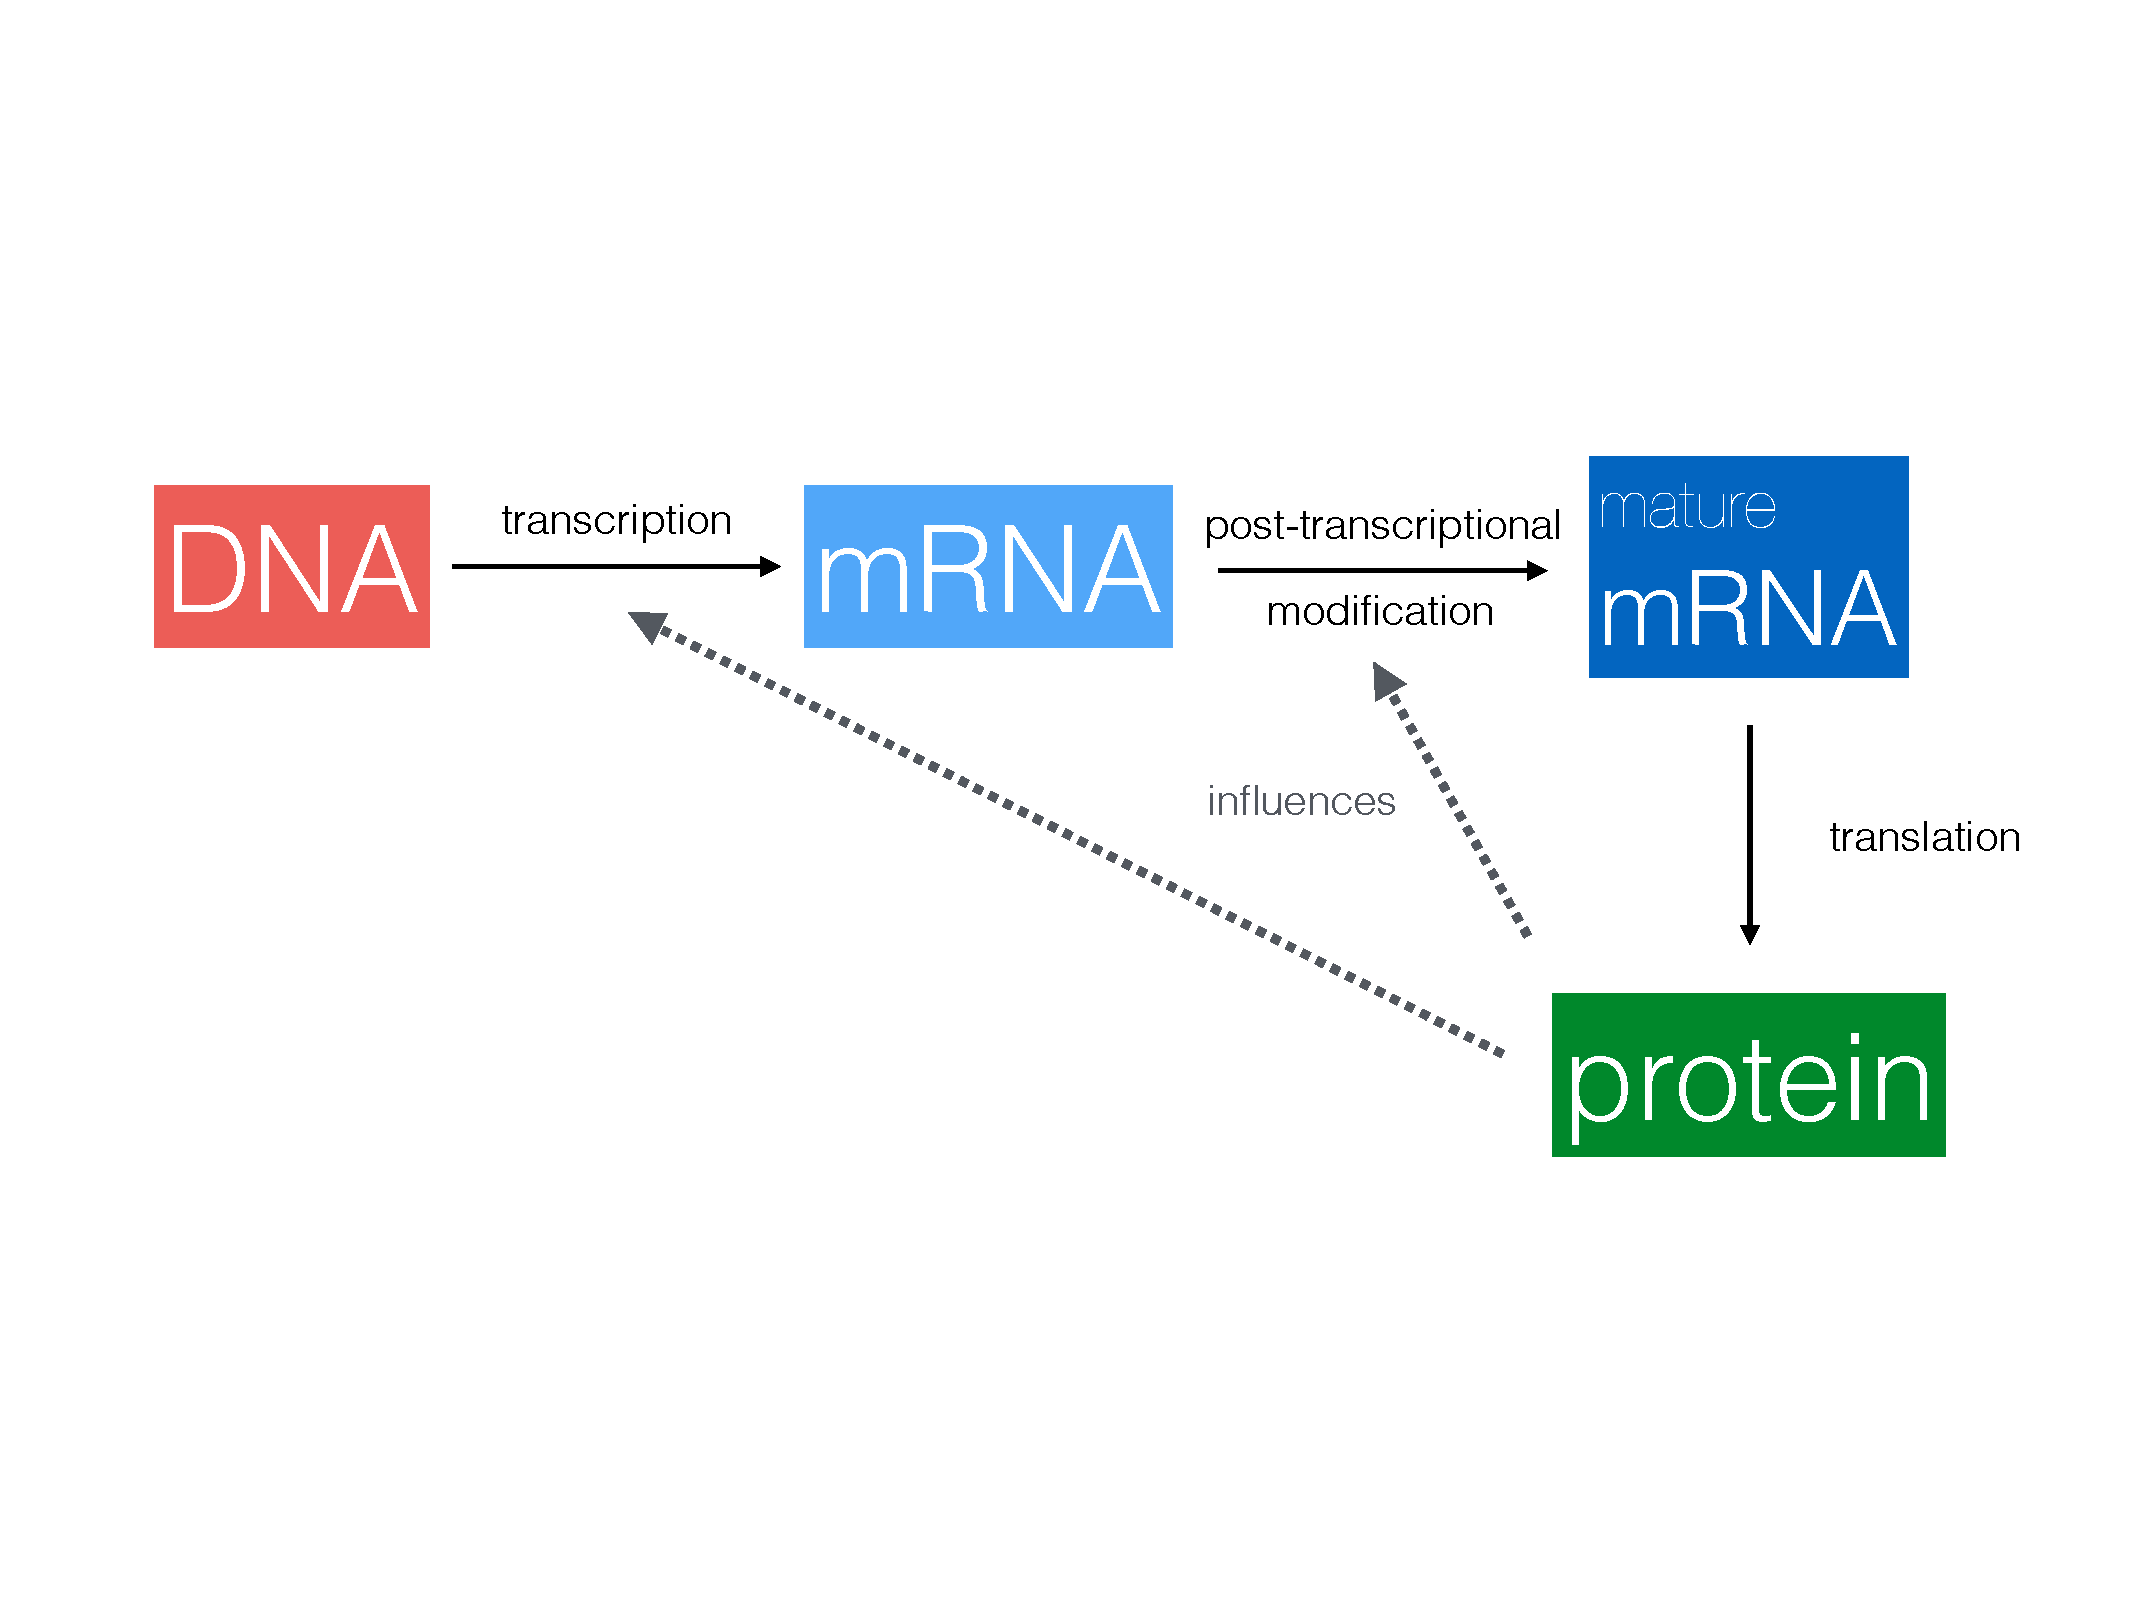
\includegraphics[width=0.69\textwidth]{pics/dogma-bio.pdf}
  \caption{Gene expression. The central dogma of molecular biology states that genes on DNA are transcribed to mRNA which is transformed to mature mRNA by post-transcriptional modifications such as splicing. The mature mRNA is then translated to proteins. This final product which plays a central role in the functions of cells in turn also influences the transcription step as well as the post-transcriptional modification step.}
  \label{fig:gene-expression}
\end{figure}

Each step during gene expression outlined above happens at a different time scale therefore when interpreting biological data it is important to keep this in mind; as the effect one sees on say gene expression at a given time might be due to a protein interaction process which took place at an earlier time point. The time scale can vary from seconds for proteins \citep{Herce:kq} up to $16$ hours for the largest gene \citep{Tennyson:1995dl}. This of course becomes even more complicated once interactions between the different players are accounted for.

It has been found that daughter cells in addition to inheriting genetic information from parent cells also inherit information that determines the characteristics of the cell unrelated to DNA, i.e. daughter cells of a cell in lungs will remain lung cells. The umbrella term often used to describe all types of material that could pass on this information not directly part of DNA is \emph{epigenetic material}. The final word on epigenetics has yet to be spoken but two types of information passed on in this manner are: Firstly the chromatin structure which determines active and inactive genes and to some extent the way they are read off. Secondly DNA methylation which is the addition of a methyl group to certain bases in DNA, altering expression of genes. 

Biological changes in state which are the focus of this work can be described in many different ways. Some changes in state are due to changes in gene expression. Other changes in state can also be epigenetic without direct changes in gene expression. Although both of these types of state changes are deeply interlinked they can occur at vastly different time scales. Here we will focus on state changes directly due to changes in gene expression.  

Further information on the cell in general as well as epigenetics can be found in \cite[Chapters~1,7]{Alberts:2007tv}. A specific overview of epigenetics has been attempted in \cite{Goldberg:2007tl} and its effect on gene expression in \cite{Gibney:2010ws}. 

\subsection{Cancer Biology}
\label{sec:cancer-biology}

An area of biology that is of great importance due to its impact on every day life and where state changes play a critical role is the study of cancer. Cancer is an extremely complex disease and attempts have been made to determine basic underlying principles, which the authors refer to as the 'Hallmarks of cancer' \citep{Hannah:2000wo, Hanahan:2011gu}. Genetic aberrations play a central role in this disease as many carcinogens (agents that can cause cancers) directly influence DNA sequences or are themselves mutations of genes naturally occurring in the cell. These defects range from point mutations on single base pairs all the way to deletions of large sections of DNA. Especially the process of cell division is highly susceptible to causing such anomalies; in healthy cells there is a DNA repair mechanism in place that prevents  changes from becoming permanent or leads to apoptosis (programmed cell death) if repair is impossible. 

One important principle shared among cancer types is the unbound proliferation of cells leading to the build up of concentrated cell masses, also known as tumours. Note that many such tumours are benign since they do not transform into cancers. The bodies defence mechanisms against such unchecked proliferation are circumvented either by introduction of oncogenes or mutations in tumour suppressor genes. Oncogenes can either be mutations of genes in the cell or genes expressed at a high level, causing an imbalance in the interactions between genes and proteins responsible for cell division. Alternatively mutations can occur in genes responsible for onset of apoptosis or DNA repair. Genetic mutations are especially problematic if they occur in the germline as the genetic material from the germline is passed on to any offspring and can lead to hereditary sensitivity to cancer.

It is important to note that one mutation or defect is not sufficient to lead to the development of cancers in fact several processes need to be affected. Additional processes developed by cells to defend against invading cancers include: A limit on the number of times a cell can differentiate. Cells also rely on external growth signals to start differentiation as well as external growth inhibition signals to stop differentiation. Cancers are known for an uninhibited expansion they of course need nutrients and therefore develop the ability to initiate the deployment of additional blood vessels. Tumorous cell become especially dangerous if they develop the ability to brake off from the main tumour and invade surrounding organs, tissues or even distant parts of the body.

As mentioned above an oncogene is a gene that can cause cancer and the first such oncogene (v-Src) was discovered in the late 1970s and early 1980s \cite{Martin:2001jx} after the initial discovery almost 70 years earlier that it was possible to induce solid tumours in chicken using a filtered agent by \cite{Rous:1911uf}. This discovery of v-Src was made investigating the Rous sarcoma virus in chicken. It was determined that a variant of v-Src, called c-Src is also contained in normal chicken. This discovery  fundamentally changed the understanding of cancer which was until then considered to be viral. Later it was determined that this gene is also found in humans and it is probably the most widely studied oncogene; despite which there remain many unknowns. The protein from this oncogene has many downstream interactions with numerous other proteins. Hence it is not surprising that in almost $50\%$ of tumours originating in breast, colon, liver, lung and the pancreas the c-Src interaction pathway has been found to be activated \cite{Dehm:2013fr}. Due to mutations c-Src is overexpressed and activated leading to the constant activation of downstream interactions linked to survival, proliferation and invasion leading to development of cancers.

Further details on cancer biology and the role of genes can be found in \cite{Weinberg:2013uu}. 

\subsection{Stem cells}
\label{sec:stem-cells}

Central to development is the creation of distinct differentiated cell types from a small collection of undifferentiated cells in the embryo. Clearly this transformation involves state changes on the genetic and epigenetic level. In recent years there has been an increase in research in these areas especially due to its potential in applications to personalised medicine; the next big frontier in medicine. The idea is to enable induction of alternative cell fates from embryonic cells or to enable development of cells that allow for a change in cell fates of tissues or blood samples. Examples include the development of neurons from cells that are responsible for creating extra cellular matrix known as fibroblasts \citep{Vierbuchen:2010fa, Pang:2011ce} or the development of muscle cells from fibroblasts \citep{Ieda:2010ir, Efe:2011bpa}.

All types of undifferentiated cells that can produce differentiated cell types are comprehensively known as stem cells (SC). Another property shared by all stem cells that they can differentiate to produce more stem cells multiple times. Broadly speaking there are two types of stem cells. Embryonic stem cells (ES cells) are cells derived from an embryo in its early development and  adult (or somatic) stem cells which are found in fully developed organs. The main difference between the two types is how many types of cells they can differentiate into. ES cells are pluripotent i.e. they can differentiate into many possible cell types. Adult SCs can only differentiate into limited cell types often serving the function of replenishing damaged cells of a single organ. For medical applications of course ES cells are more useful, but for some people there are ethical concerns associated with their usage; independently of the rational behind these concerns they do create issues in research.

A new approach was proposes by \cite{Takahashi:2006hi} to use differentiated somatic cells and derive induced pluripotent stem cells (iPS cells) which have distinct advantages if successful. These iPS cells are able to differentiate to various cell types and could in future allow for personalised medicine. The process in creating iPS cells involves artificially inducing $4$ genes (reprogramming factors) for several days and they do indeed find cells which have properties comparable to ES cells. More detailed studies show that iPS are influenced by the used reprogramming factors and there are epigenetic differences between ES and iPS \citep{Carey:2011bs, Bock:2011kx}. One important concern is the difference in DNA methylation of iPS cells and ES cells, this problem is now being addressed \citep{Bagci:2013ey} as well as other safety concerns.

Further information on Stem cells, ES cells, somatic cells as well iPS cells, can be found in \cite{lanza2009essentials} and in \cite{Lanza:2013uk}. 

\subsection{Cell cycle}
\label{sec:cell-cycle}

An essential step in all topics outlined above as well as any state change is the cell cycle. In simple terms it is the process by which two daughter cells is are produced from one mother cell by duplication of the cell contents; most importantly the DNA. Details of the process can vary between organisms as well as between different stages of development. Most cells in the human body are not taking part in the cell cycle, but are in a resting phase. The most basic principles of the mammalian cell cycle can be summarised into four phases:

\begin{itemize}
\item {\bf G$_1$ phase} The first gap phase during which cells increasing in size. It also includes a restriction point up to which the cell is driven by external stimuli and after which it can progress through G$_1$ independently. 
\item {\bf S phase} The transition from the G$_1$ to the S (Synthesis) phase contains a powerful checkpoint after which the cell is committed to duplication. During the S phase itself DNA is replicated.
\item {\bf G$_2$ phase} The second gap phase is not present in all organisms. In short the cell keeps increasing in size synthesises proteins and prepares for mitosis. It contains a checkpoint to determine DNA damage and stops the process. 
\item {\bf M phase} The final step in the cell cycle is the mitotic (M) phase. The duplicated chromosomes are separated into two cells and a new nucleus is created. The M phase also contains a checkpoint to ensure the cell is ready for division.
\end{itemize}

Despite all these checks and balances in place during the cell cycle uncontrolled cell doubling is still a concern in tumourigenesis as mentioned above. Intervention on the cell cycle plays a central role in unbound growth of cells. In many cases proteins essential during check points are mutated, inhibited or overexpressed \citep{Williams:2012eg}. Understanding and perturbing elements in the cell cycle could be a good approach for potential cancer treatments since the mammalian cell cycle is conserved across a variety of cell types; at the same time it plays a central role in cancers. 

The cell cycle is also sensitive to UV radiation which is a well known carcinogen. UV radiation incident on a cell can lead to damage to DNA if the damage is too extensive cells can lead to apoptosis. If the damage is not too large some cells will arrest and re-enter the cell cycle at a later time. Radiation has a direct effect on gene expression also related to the intensity of the ration \citep{Gentile:2003in}. 

More information about the cell cycle can be found in \cite[Chapter~17]{Alberts:2007tv} and its relationship to cancer in \cite[Chapter~8]{Weinberg:2013uu}.


\section{Experimental background}
\label{sec:exper-backgr}

In this section we explore two techniques to obtaining time-course assays for genome wide gene expression data. Current techniques for such measurement are only possible on a population level. There exist techniques for single cell measurements \citep{Buganim:2012hp}, but these techniques are not yet fully developed and only allow measurement of a limited number of genes. Initially to be able to obtain these measurements is to create a homogenate from the sample which is done by crushing cells using a variety of different mechanical procedures. After which different subsets are filtered out of the mixture to perform microarray experiments and mRNA for RNA sequencing (RNA-seq). 

\subsection{Microarray}
\label{sec:microarray}

Different stages of gene expression can be measured using microarrays, here we present the one most commonly used the DNA microarray; the aim is to measure mRNA levels. There are two types of DNA microarray, the cDNA \citep{Hughes:2001ho} and the high􏰄density oligonucleotide chips \citep{Lockhart:1996jw}. The basic principle of cDNA\footnote{Complementary DNA, DNA reverse-transcribed from mRNA} microarrays is based on high-density array with DNA sequences printed on them. The sample mRNA reverse-transcribed to cDNA labelled in two different colours. Equal proportions are mixed together and hybridised to the array and using a scanner fluorescence measurements are made for each colour. The resulting expression is obtained by the ratio of the measurements in each colour, see \cite{phimister1999chipping} for further information. To ensure measurements are comparable between different samples and even different experiments it is important to normalise each sample. The most robust normalisation method is to based on subtracting a position and intensity ($A$) dependant constant from the log ratios of the intensity measurements in green $G$ and red $R$:

\begin{equation}
  \label{eq:microarray-norm}
  \log_2 \frac{R}{G} - l(A, j), 
\end{equation}
where $l(A, j)$ is the lowess fit \citep{Cleveland:2012fu} to the plot of $\log_2 R$ against $\log_2 G$ rotated counterclockwise by $45^{\circ}$. More detail on normalisation and cDNA microarray measurements can also be found in \cite{Dudoit:2002va}. 

\subsection{RNA sequencing}
\label{sec:rna-sequencing}

Until recently the most prevalent method for obtaining gene expression data which is essential to understanding disease states has been DNA microarray measurement. One drawback is that observations are relative and indirect i.e. measurements via fluorescence intensity and ratio of two colours. Additionally microarray measurements are limited by prior knowledge of genes, since arrays can only be constructed to include sequences of known genes. A new contender that attempts to address some of the shortcomings of these is RNA-seq developed roughly $5$ years ago \citep{Mortazavi:2008jj, Nagalakshmi:2008cj}. RNA-seq measurements are integer count data and cover the whole genome. 

\subsubsection{Experimental protocol}
\label{sec:technique-bio}

RNA-seq experiments also attempt to measure mRNA obtained from homogenate. The first step is a random fragmentation of the sample mRNA. The next step is a reverse-transcription of the fragmented samples to cDNA. Next comes a Polymerase chain reaction (PCR) step which is a method of amplification to obtain more copies of DNA from few copies of a slice of DNA and is performed multiple times. This step is the source of one type of systematic error since different sections of  DNA have a different susceptibility to a PCR amplification. In the next step each fragment is sequenced in high throughput machine; resulting sequences are referred to as \emph{reads}. These reads can now be mapped to a known genome or transcriptome\footnote{collection of all RNA} resulting for one count for each fragment of gene found;  alternatively reads can also be used to construct a transcriptome without mapping it to a known genome (de novo assembly). Figure \ref{fig:li-biostats} from \cite{Li:2012ea} summarises this protocol. 

\begin{figure}
  \centering
  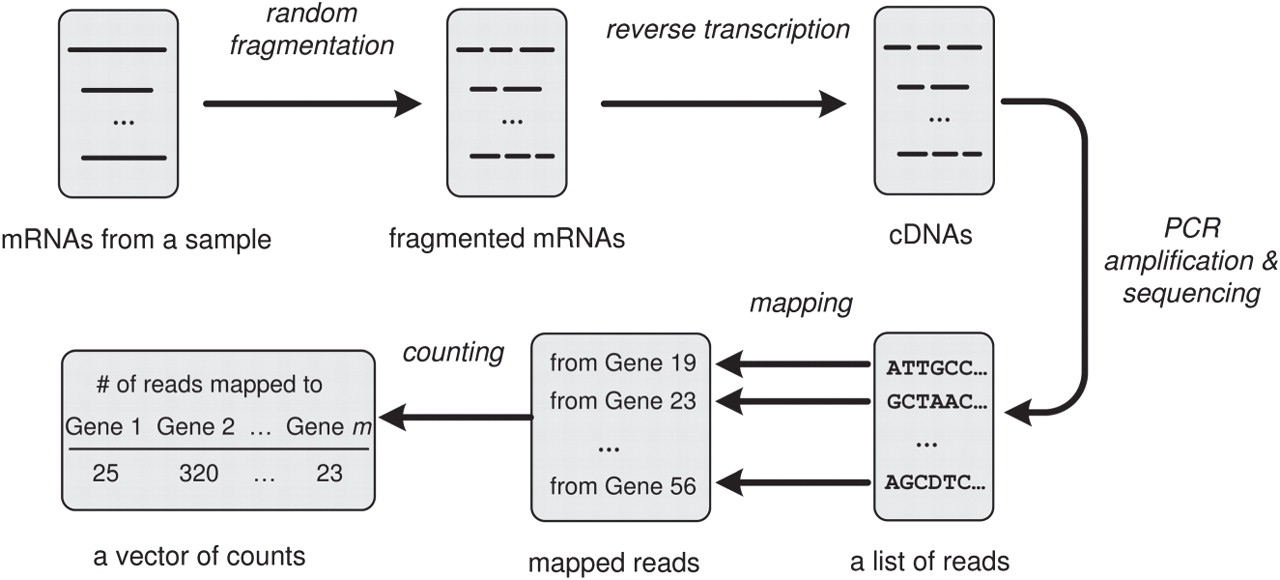
\includegraphics[width=0.9\textwidth]{pics/li-biostats12.jpg}
  \caption{RNA-sequencing (RNA-seq). The most commonly used modern genome wide assay. From a homogenate cell sample mRNA is filtered out and passes through this pipeline to give integer count expression values for genes. Figure from Li et al., Normalization, testing, and false discovery rate estimation for RNA-sequencing data, Biostatistics, 2012, 13(3), by permission of Oxford University Press.}
  \label{fig:li-biostats}
\end{figure}

\subsubsection{Normalisation}
\label{sec:normalisation}

Though RNA-seq avoids some of the issues associated with microarray measurements it still has it's own difficulties that need to be overcome before analysing the data. The first as, already mentioned above, is the systematic error due to the PCR step. Another is due to the random fragmentation step; since larger genes will have more fragments resulting in a higher per gene count. Due to these reason the total number of counts is also not conserved across different samples. 

Therefore there is a real need for a normalisation step prior to comparison of data, to ensure the affect of these problem are minimised. The issue of different gene lengths can be removed by simply normalising for gene length which is a known quantity when  mapping counts to a genome. Additionally this is only an issue when comparing genes in the same sample. For comparisons between samples this step is unnecessary since gene length is constant across samples. The question normalisation between samples especially arises in differential expression. In RNA-seq data unlike for microarray data the question of normalisation has yet to be settled. The normalisation method most commonly used is to normalise all samples to a fixed number of reads, but this leads to issues as can be illustrated using a simple example. 

Say $N_{ij}$ is the total number of reads in experiment $i$ for gene $j$. In a simple case $N_{1j} \simeq 2 \, N_{2j}$ for all genes and hence sequencing depth of experiment $2$ twice the sequencing depth of experiment $1$. In a slightly more complex example the issue becomes clear. If we now consider $j = 1, \ldots,  100$ to have $N_{1j} = 1$ and $N_{2j} = 2$ and for $j = 101$ $N_{1j} = 100$ and $N_{2j} = 0$ both experiments have the same sequencing depth which would suggest all genes are differentially expressed. But it would be more realistic to consider that the sequencing depth of experiment $2$ is twice that of experiment $1$ and that only gene $j = 101$ is differentially expressed. Therefore a good strategy would be identify genes that are not differentially expressed and calculated a sequencing depth just for those and use it for the whole sample. One idea would be to identify housekeeping genes\footnote{genes that are supposed to remain constant} for the particular application at hand and calculate a sequencing depth; but this is an unsatisfactory solution since it does not generalise (each application would have different housekeeping genes) and requires further experiments or prior knowledge. \cite{Bullard:2010go} propose a method using quantiles instead of total counts. \cite{Robinson:2010dd} propose a method based on total count normalisation called trimmed mean of M values (TMM). The idea is to impose a cutoff on log-fold change $M$-value and the absolute expression level $A$-value and calculate the sequencing depth using what remains. The $M$-value  and $A$-value is calculated as follows:

\begin{eqnarray}
  \label{eq:MA-values}
  M_j &= \log_2 \frac{N_{ij} / N_i}{N_{i'j}/ N_{i'}} \\
  A_j &= \frac{1}{2} \log_2 \left(N_{ij}/ N_i \bullet N_{i'j} / N_{i'} \right).
\end{eqnarray}

In the R package \texttt{edgeR} this method as well as a few other have been implemented for application to RNA-seq data \cite{Robinson:2010cw}. 
A summary comparing different normalisation methods can be found in \cite{Oshlack:2010kr}. 

%%% Local Variables:
%%% TeX-master: "warwickthesis"
%%% End:

